\chapter{Event Selection\label{ch:selection}}

This chapter discusses additional event-wide requirements imposed to further
improve the sensitivity of selecting the signal of interest over the background contributions
beyond that of the preselection requirements covered in Chapter~\ref{ch:objects}.
Event classification is covered in Section~\ref{sec:classification}, in which two classes of
events are defined for extracting signal separately.
Section~\ref{sec:higgsreconstruction} discusses how the photons and jets passing the preselection
requirements are assembled into Higgs candidates. For the resonant search $X\rightarrow HH$,
Section~\ref{sec:Xreconstruction} discusses how the two Higgs come together to construct a resonant
candidate. Finally, the construction of a data control
sample, discussed in Section~\ref{subsec:dataCS}, allows for the study of additional event-wide
requirements for improving sensitivity, discussed in Section~\ref{sec:extraction}.

\section{Event Classification\label{sec:classification}}

B-tagging, presented in Section~\ref{subsec:btag}, is used at the preselection level by
requiring 1 CSVL b-tagged jet. To further improve the sensitivity, the working point used for
signal extraction is the medium one (CSVM), which corresponds to an efficiency of around 60--70\%
and a mistag rate 1--2\%, depending on the jet $p_{\rm T}$.
There is also a tight working point (CSVT) not used in this analysis,
which corresponds to a mistag rate of 0.1\%.
With the CSVM working point, events are classified into three categories for the resonant search
based on the number of CSVM b-tagged jets. Events with two or more b-tags, called high purity,
drive the sensitivity of the search. Events with one b-tag, called medium purity,
bring low contribution to the sensitivity
but allow for increased signal acceptance. Events without any b-tags,
called low purity, are used only for cross-checks and are rejected from the main analysis.
The preselection cuts and event categorization
are summarized in Table~\ref{table:gencut}.
For the nonresonant search, the high and medium purity categories will be further divided based
on the four-body mass spectrum, discussed in Section~\ref{sec:}

\begin{table}[ht]
  \centering
  \renewcommand{\arraystretch}{1.4}
  \caption{Summary of the selection applied to photons and jets and the event classification
for the resonant search.}
  \begin{tabular}{|c|c|c|}
\hline
Photons & Jets & Classification \\
\hline
tight photon identification                        & loose jet identification  & \\
$p_{T \gamma_1}/ \Mgg > 1/3$  & pileup rejection   & \\
$p_{T \gamma_2}/ \Mgg > 1/4$  & $p_{T j} >25$~GeV  & \\
$|\eta_{\gamma}|<2.5$                              & $|\eta_{j}|<2.5$  & $\ge$~2 CSVM b-tags \\
$ 100 < \Mgg < 180$~GeV                 & $\ge$~1 CSVL b-tag & exactly 1 CSVM b-tag \\
\hline
\end{tabular}

  \label{table:gencut}
\end{table}

\section{Higgs Reconstruction\label{sec:higgsreconstruction}}

From the lists of photons and jets passing the identification and kinematic requirements, Higgs
candidates are constructed. When there are more than two photon or jet candidates, a choice
must be made as to which pair is consistent with the decay of a Higgs. In the case
of choosing the diphoton candidate, the two photons with the highest $p_{\rm T}$ are chosen
as jets faking photons tend to be softer than prompt photons.

In the case of chosing the jets for the dijet candidate, four choices were considered after b-tagging:
\begin{itemize}
\item the two jets with the highest $p_{\rm T}$,
\item the pair of jets that maximizes $p_{{\rm T},jj}$,
\item the pair of jets that maximizes $\frac{p_{{\rm T},jj}}{\Mjj}$, and
\item the pair of jets which minimizes $|\Mjj-\Mgg|$.
\end{itemize}
In the high-purity category, the choice is among all b-tagged jets,
while in the medium-purity category, the
choice is among all non-tagged jets to pair with the b-tagged one.
The criterion used in this analysis is the one that maximizes $p_{{\rm T},jj}$. 
This choice selects the correct jets roughly 87\% of the time, and it does not produce any local peaking
structure in the background. For the resonant search
in the high-purity (medium-purity) category, the resolution, defined as the half-width at half-maximum,
decreases from 20 (25) GeV to 15 (15) GeV as the resonance mass increases from 300 GeV to 1 TeV.
This is also shown visually in Figure~\ref{fig:mjj_onlyhiggs}.

\section{Resonance Reconstruction and Kinematic Fit\label{sec:Xreconstruction}}

For the resonant, the double Higgs system is constructed
by combining the $\Hgg$ and $\Hbb$ candidates. (This is also used in the nonresonant search
where the resulting mass distribution does not correspond to a local peak.)
In order to improve the resolution on the $\Mggjj$ distribution, an additional constraint is imposed
requiring the dijet mass to be consistent with the Higgs mass. This constraint, called the
kinematic fit~\cite{Chatrchyan:2013yoa}, is performed by varying the jet four-momentum
with respect to their
respective energy and position resolutions in order to fix $\Mjj = 125$~GeV.
The resulting distribution is denoted as $\Mggjjk$. Distributions before (\Mggjj) and after (\Mggjjk)
the kinematic fit
are shown in Figure~\ref{fig:mggjj_onlyhiggs} for the resonant signal and resonant backgrounds
and in Figure~\ref{fig:mggjj_controlplot} for data and the sum of backgrounds.

\begin{figure}[ht]
 \begin{center}
   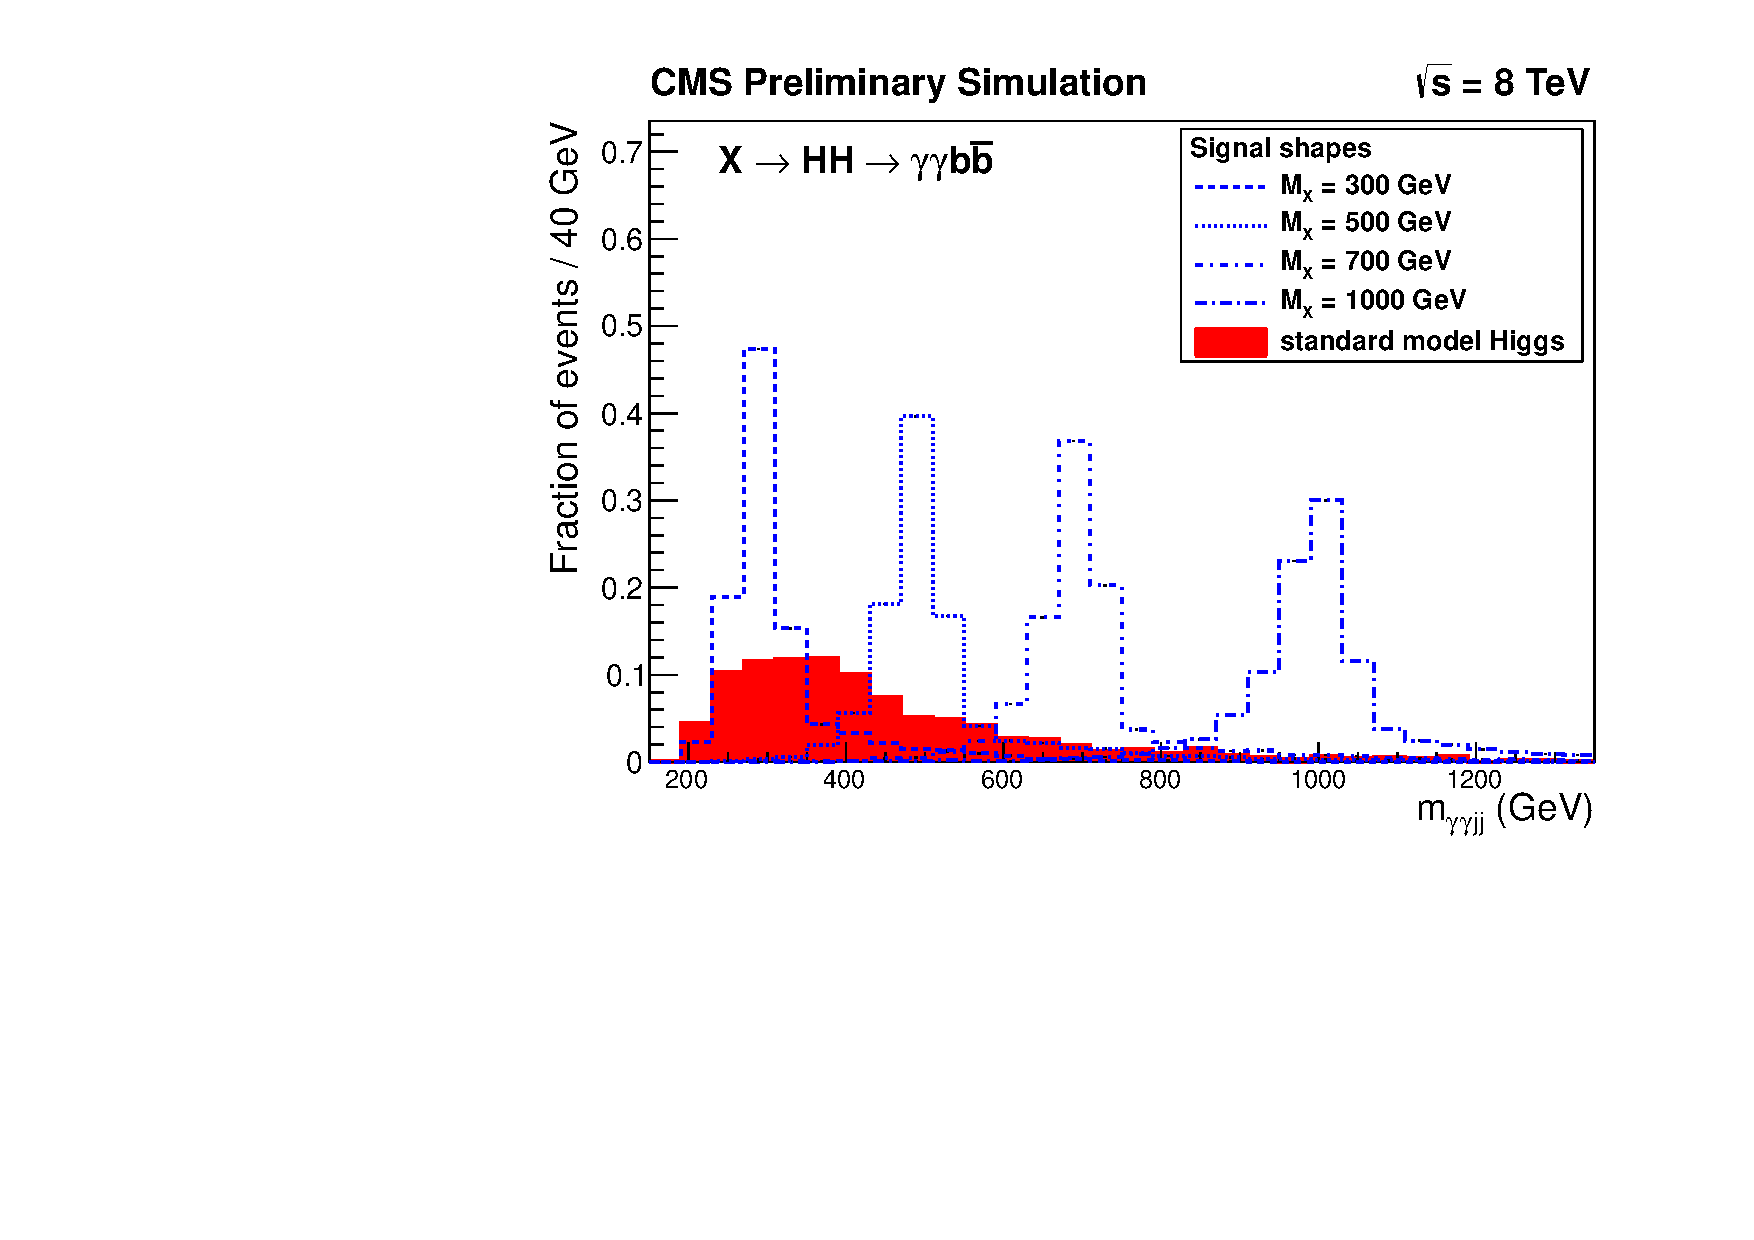
\includegraphics[width=0.70\textwidth]{figures/selection/TotalMass_OnlyHiggs.pdf}
   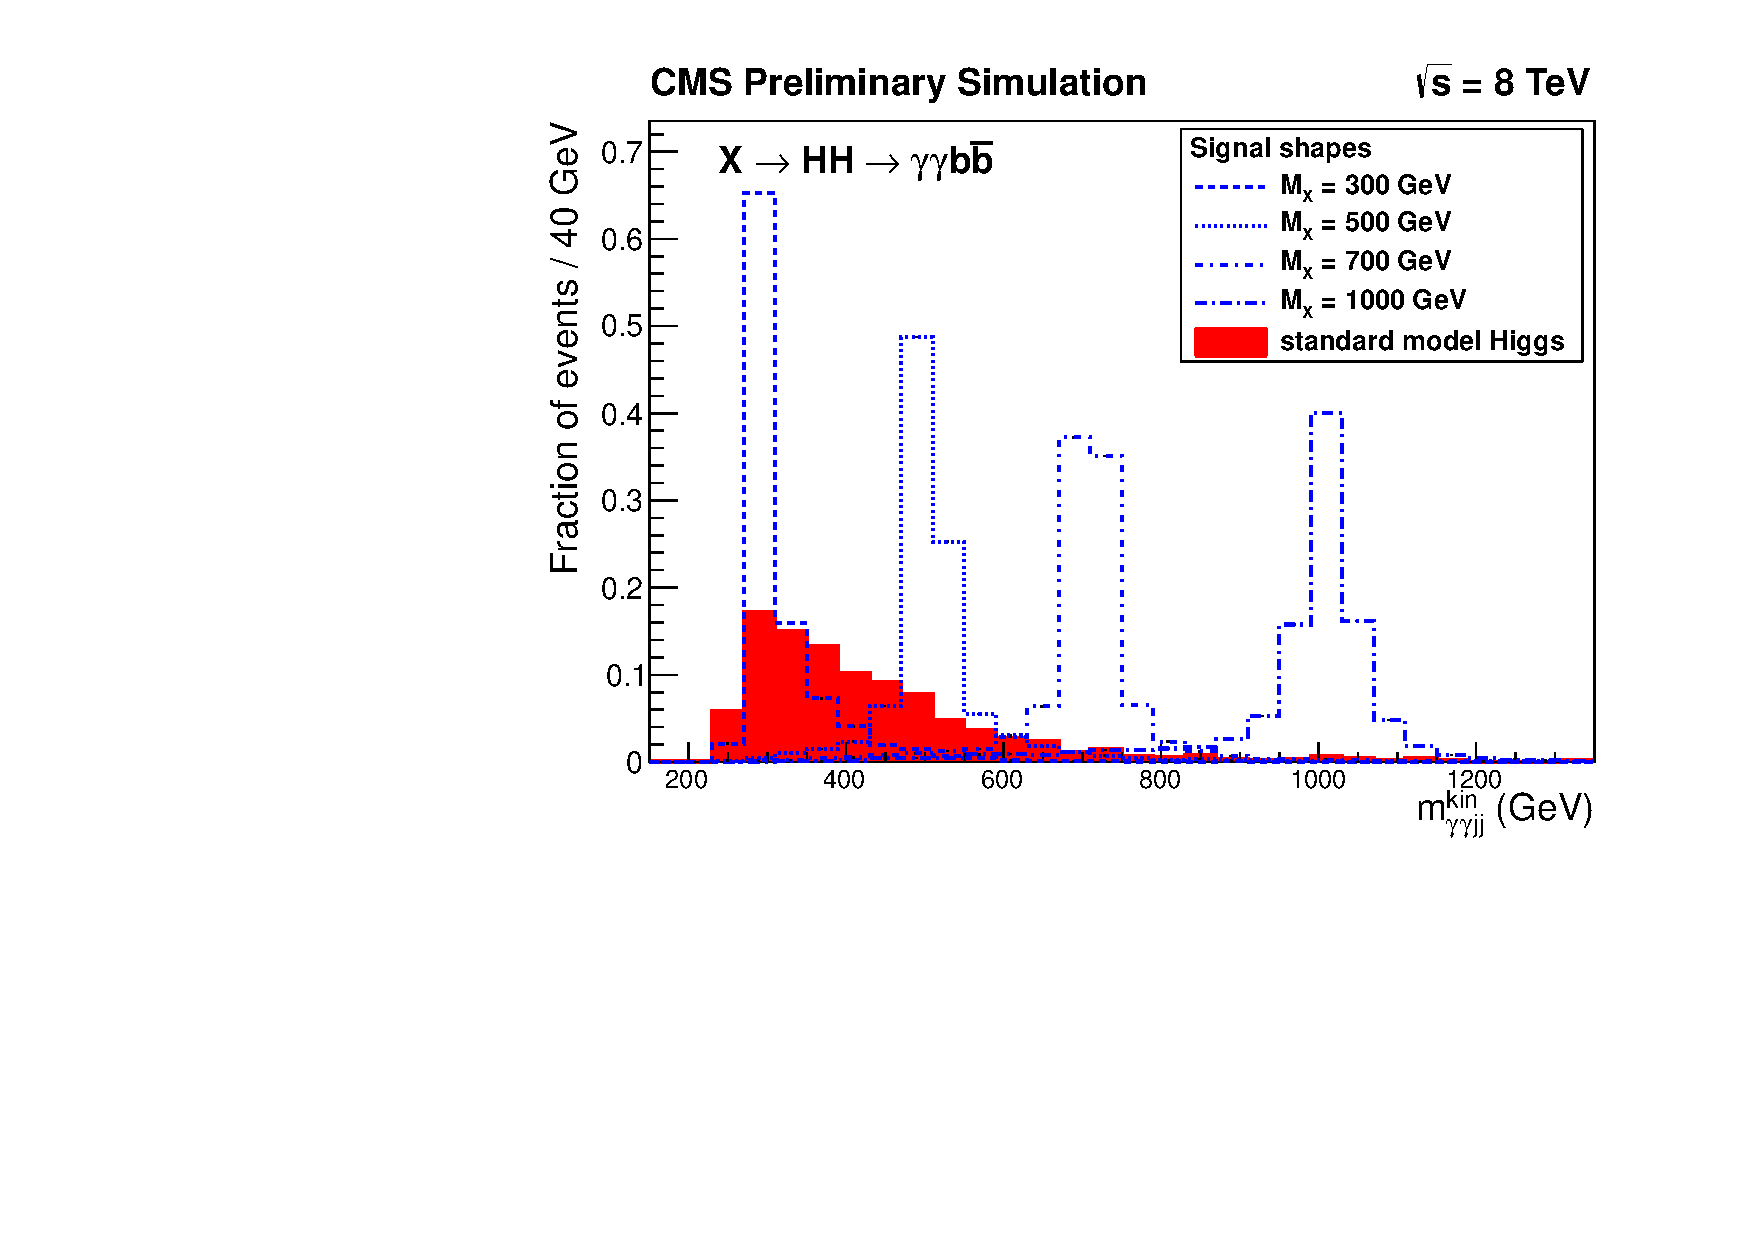
\includegraphics[width=0.70\textwidth]{figures/selection/TotalMassKinFit_OnlyHiggs.pdf}
 \end{center}
\caption{Simulated four-body mass spectrum for the resonant signal and the sum of all production
mechanisms of the
SM Higgs boson after basic selections on photons and jets and requesting at least
one loose b-tagged jet. Before (after) the kinematic fit is shown in the top (bottom) figure.
The spectra are normalized to one.}
\label{fig:mggjj_onlyhiggs}
\end{figure}

\begin{figure}[ht]
 \begin{center}
   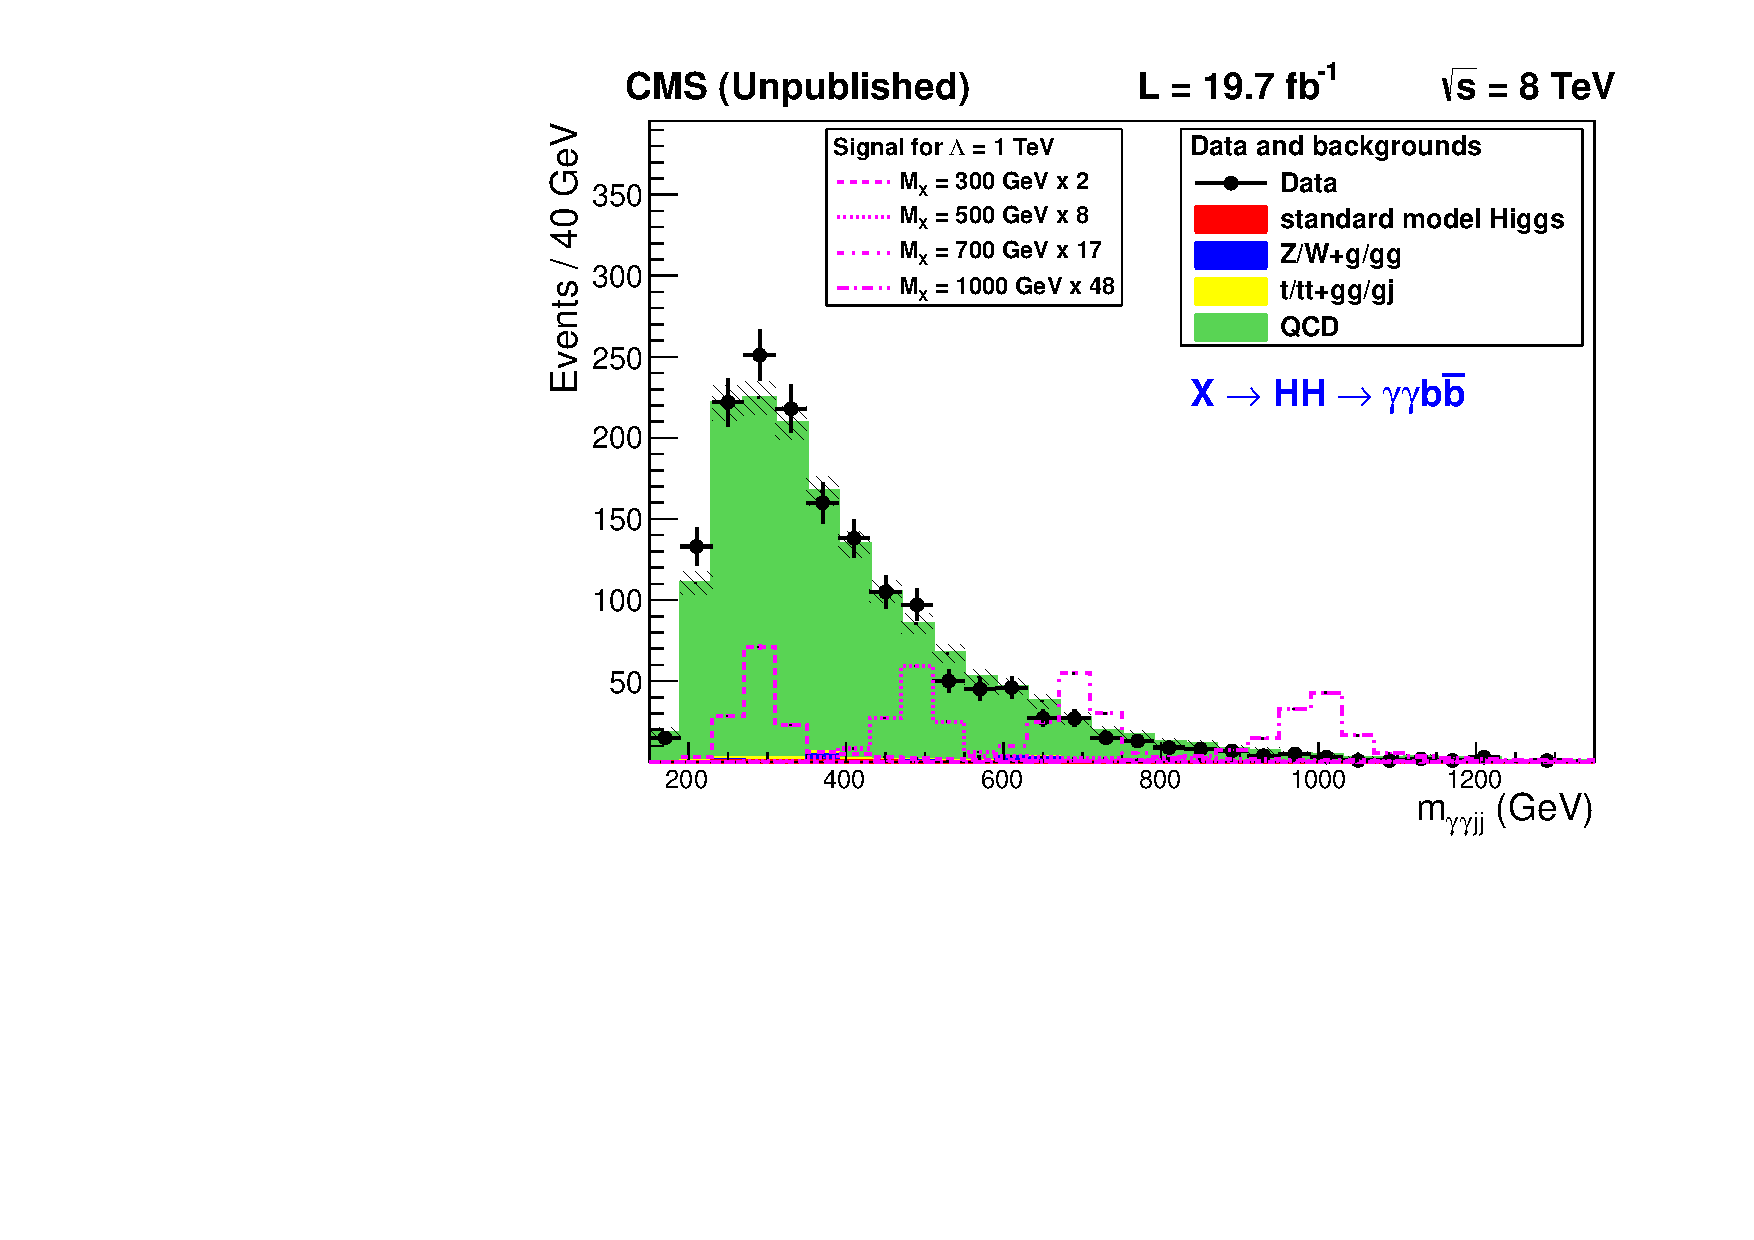
\includegraphics[width=0.45\textwidth]{figures/selection/TotalMass_ShapeNormalized_sys.pdf}
   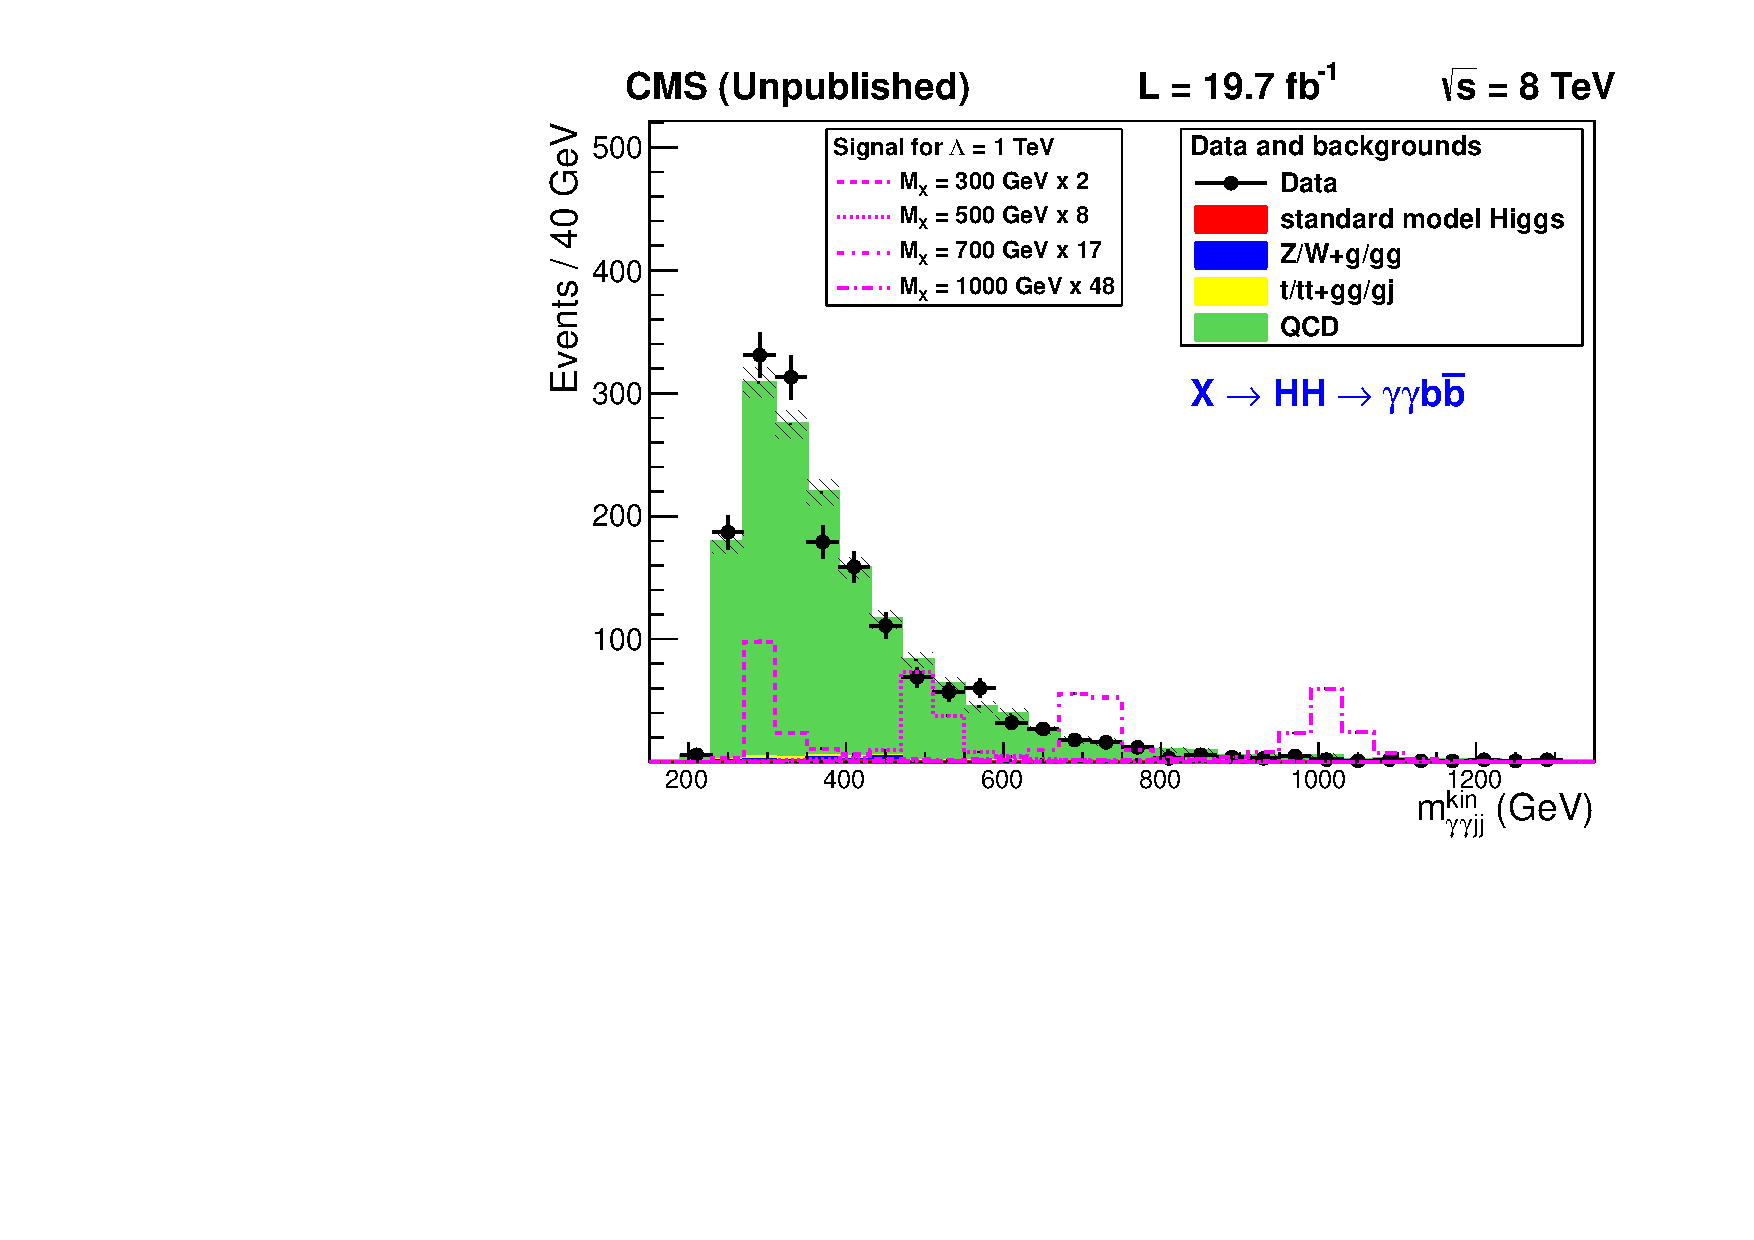
\includegraphics[width=0.45\textwidth]{figures/selection/TotalMassKinFit_ShapeNormalized_sys.pdf}
   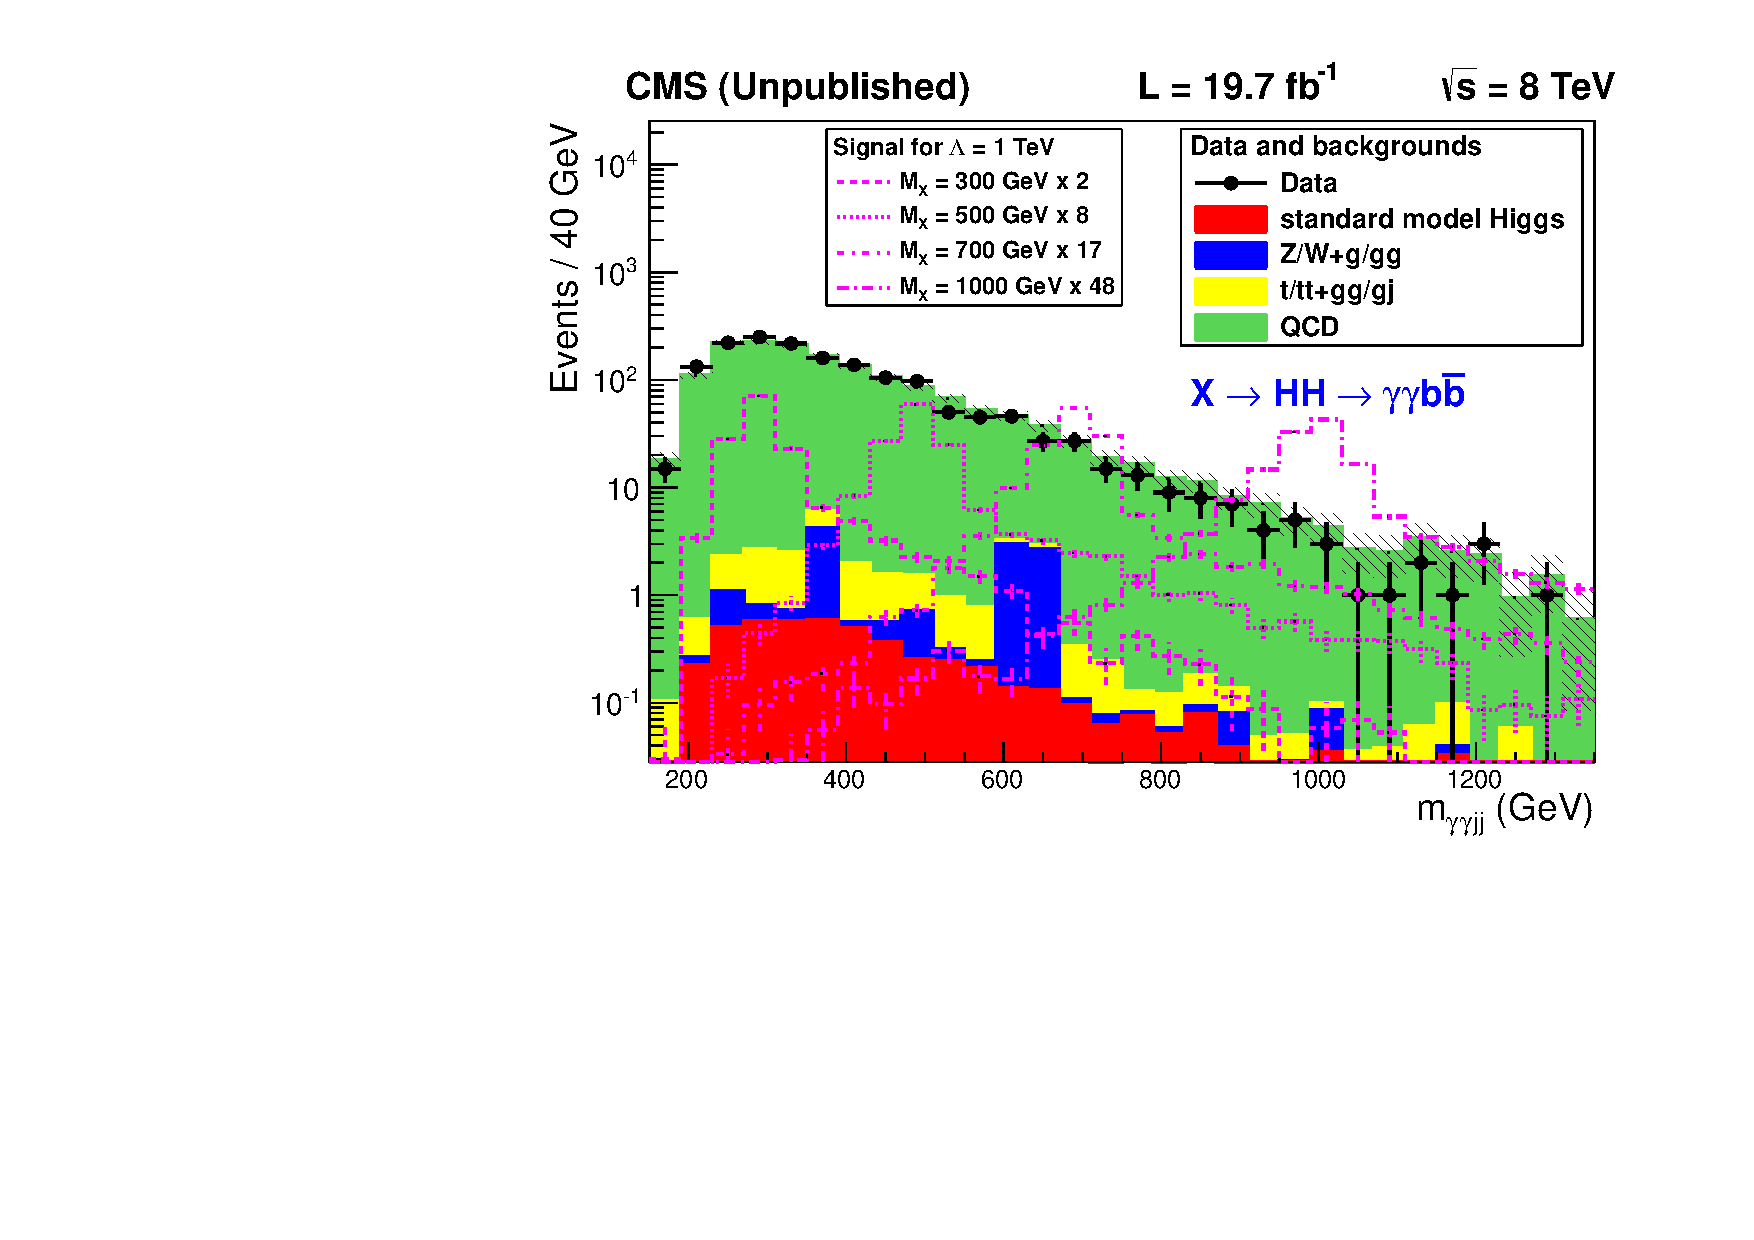
\includegraphics[width=0.45\textwidth]{figures/selection/TotalMass_ShapeNormalized_Log_sys.pdf}
   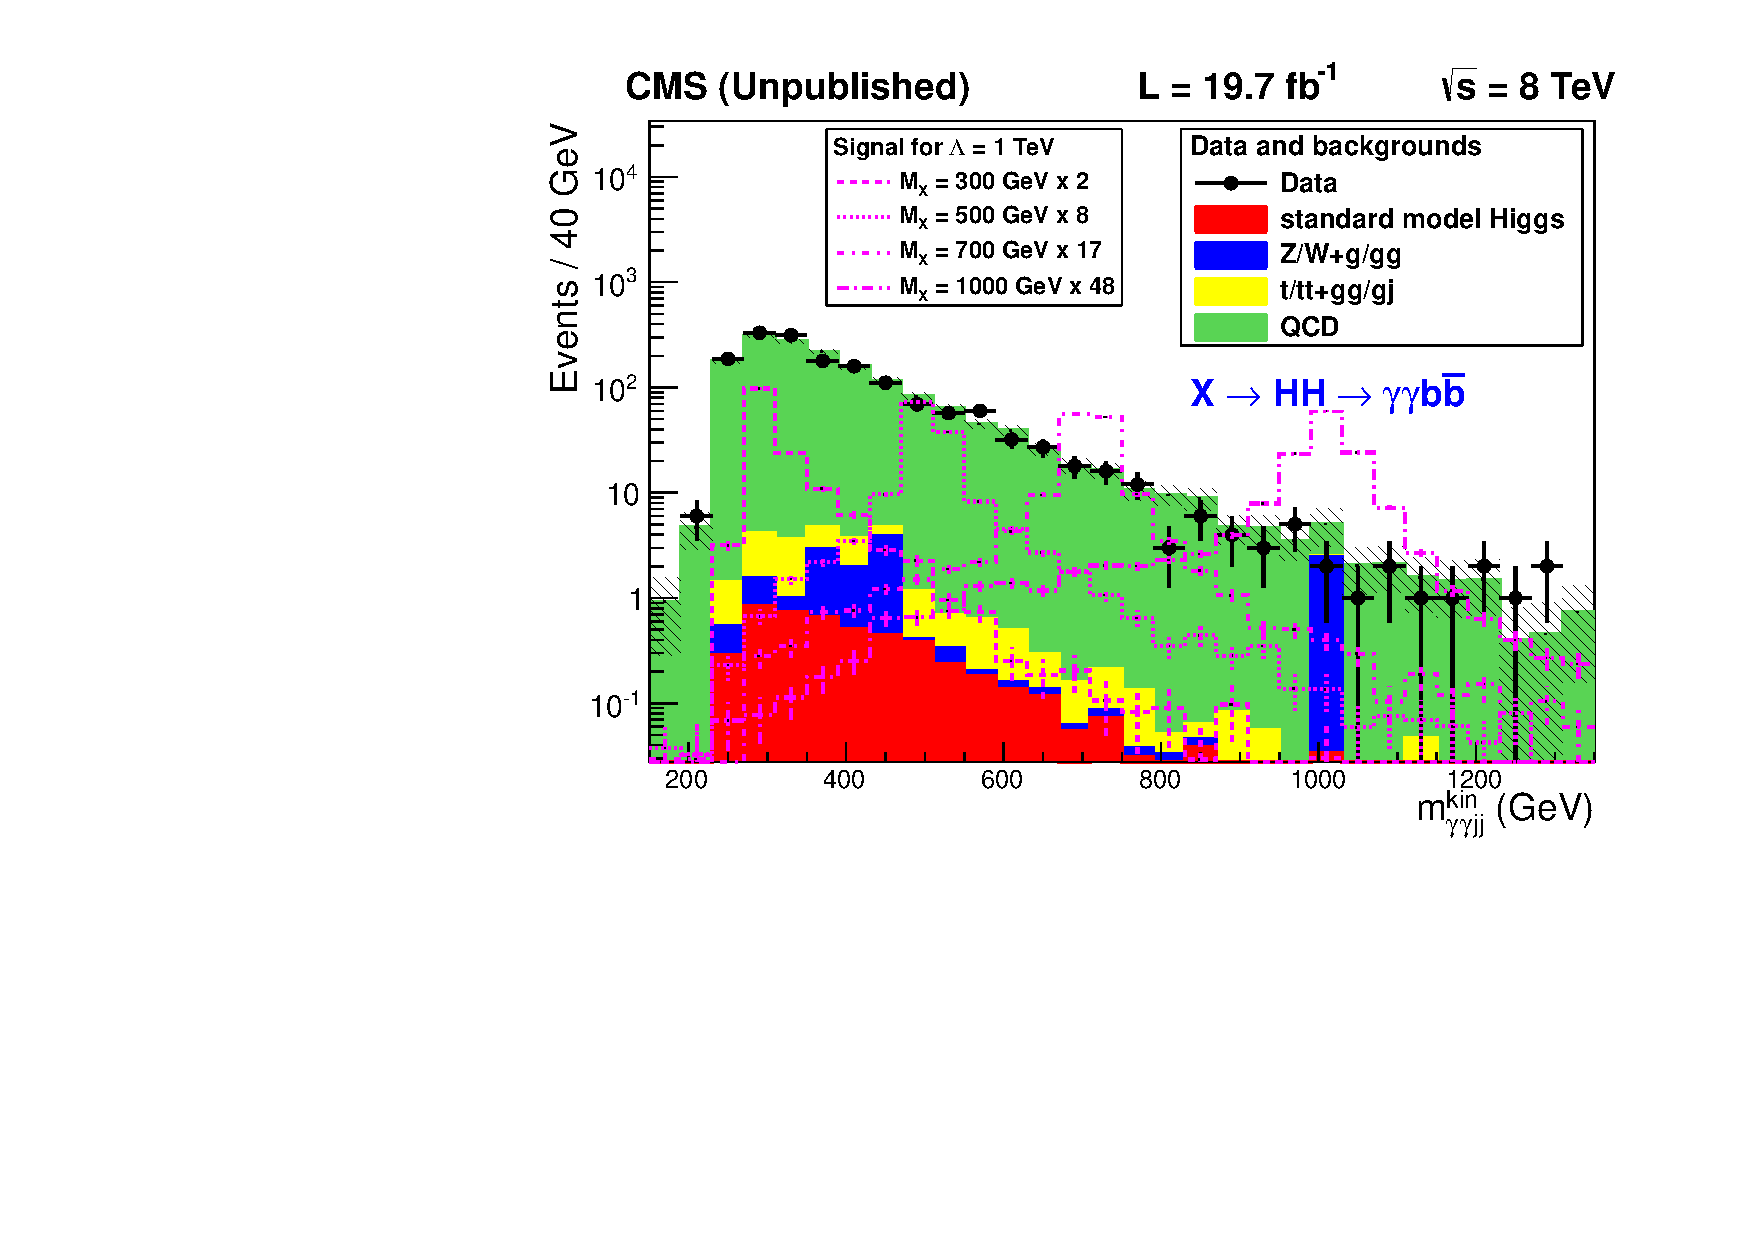
\includegraphics[width=0.45\textwidth]{figures/selection/TotalMassKinFit_ShapeNormalized_Log_sys.pdf}
 \end{center}
\caption{Control plots for the four-body mass spectrum after basic photon and jet selections
and requiring at least one loose b-tagged jet. The simulation is normalized to data and
the statistical uncertainty on the number of simulated events is shown in dashed overlay.
The left (right) figures are before (after) the kinematic fit is imposed, and
the top (bottom) figures are shown in linear (log) scale.}
\label{fig:mggjj_controlplot}
\end{figure}

\section{Signal Extraction\label{sec:extraction}}

The strategy for extracting a measurement of the signal yield centers on the fact that there
are three spectra, $\Mgg$, $\Mjj$, and $\Mggjjk$, from which an excess can be measured.
For the resonant search, an excess would appear as a localized bump on the
$\Mggjjk$ spectrum giving a direct handle on $m_X$,
but, recalling from Figure~\ref{fig:mggjj_controlplot}, there is a kinematic peak in the background
around 300 GeV. In order to avoid looking for a peak on top of a peak, the resonant search is
divided into two regimes:
\begin{itemize}
\item the high-mass analysis searches for an excess on the $\Mggjjk$ spectrum for $m_X \ge 400$~GeV, and
\item the low-mass analysis searches for an excess on the $\Mgg$ spectrum for $m_X \in [260, 400]$~GeV.
\end{itemize}
In both cases, there is more discrimination to be gained by imposing requirements on the two spectra
not being fit, which is described in Section~\ref{subsec:add_discrimination}.

The nonresonant search can be viewed as a special case of the low-mass resonant search in which
the $\Mggjjk$ spectrum has no local peak. Here, excess is sought on the $\Mgg \times \Mjj$ plane,
with additional requirements imposed on the $\Mggjj$ and the angle between the two Higgs candidates
$\acosthetastar$.

\subsection{Data Control Sample\label{subsec:dataCS}}

In optimize the kinematic cuts imposed after preselection, a data control sample is constructed.
The events for the sample are selected with the same preselection as data except for
the inversion of one of the photon's identification and isolation requirements, giving a sample
dominated by the contribution of $\gjjj$ rather than the $\ggjj$ of the signal region.

The main kinematic variables related to the photons have a different shape
between the control sample and the
signal region, so reweighting of the control sample is needed to ensure that the distributions
match those in the signal region. The event weights are derived by matching the shape
of the control sample to data in the $p_{{\rm T},\gamma_1} \times p_{{\rm T},\gamma_1}$ plane,
with a veto in signal region on the range $\Mgg \in [115, 135]$~GeV. Afterwards,
the normalization of the control sample is fixed to the normalization of the signal
region. Figure~\ref{fig:datacs}
shows the effect of the reweighting on the three spectra of interest.

\begin{figure}[ht]
 \begin{center}
   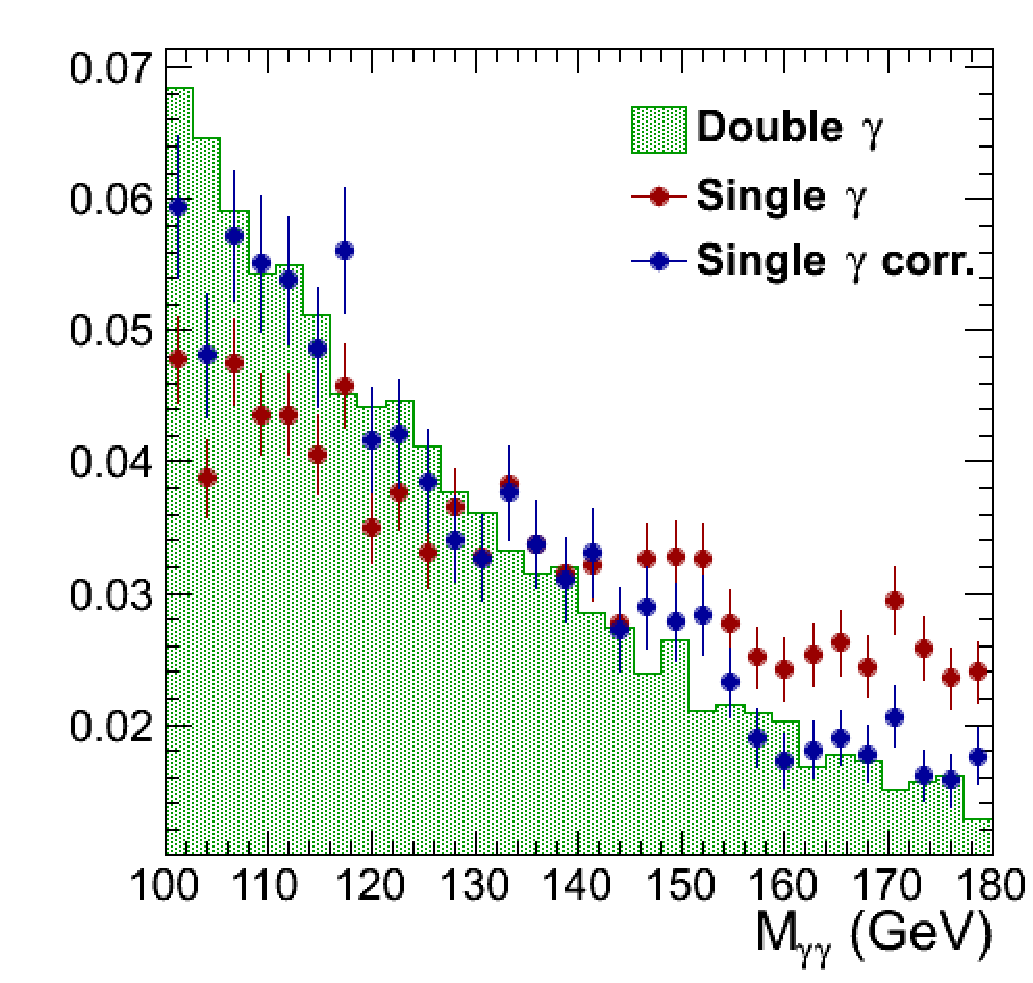
\includegraphics[width=0.45\textwidth]{figures/selection/mggSpectrum.pdf}
   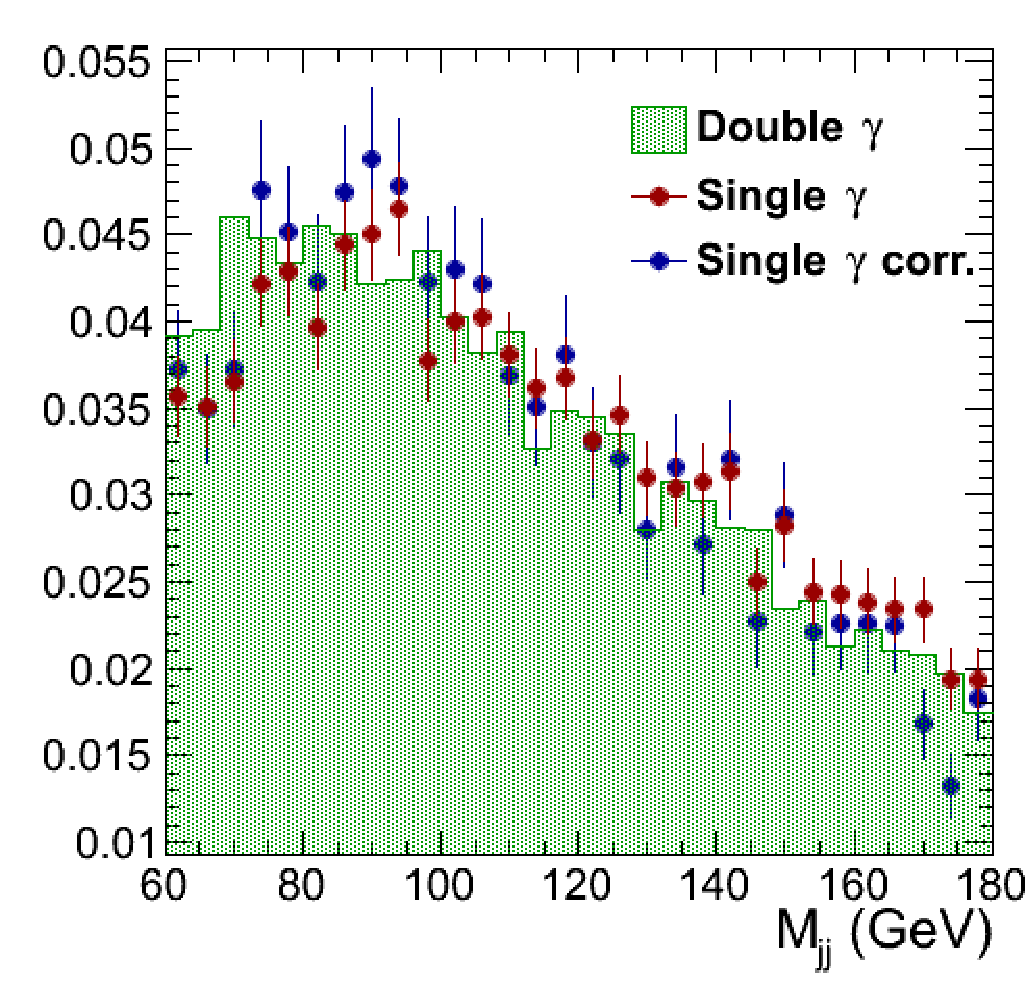
\includegraphics[width=0.45\textwidth]{figures/selection/mjjSpectrum.pdf}
   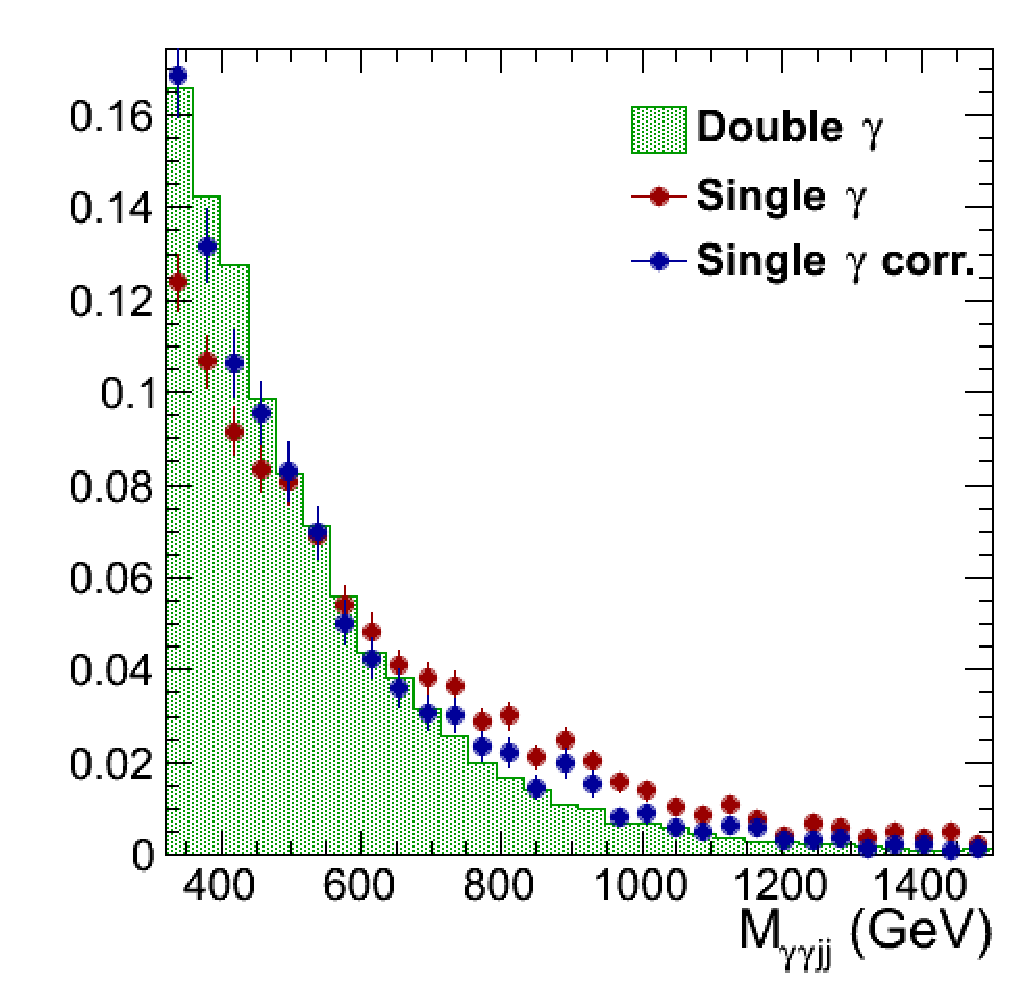
\includegraphics[width=0.45\textwidth]{figures/selection/mggjjSpectrum.pdf}
 \end{center}
\caption{The effect of reweighting the $\gjjj$ control sample
to match the kinematic distributions of the
signal region. Double $\gamma$ refers to the signal region, with a veto in $\Mgg$ or $\Mjj$
on a range about the Higgs mass. Single $\gamma$
refers to the $\gjjj$ sample before the weighting, and Single $\gamma$ corr. refers to the reweighted
$\gjjj$ sample. The shape of the reweighted $\gjjj$ sample is reasonably consistent with that of data
for all three spectra.}
\label{fig:datacs}
\end{figure}

\subsection{Additional Discrimination\label{subsec:add_discrimination}}

When searching for a high-mass resonance through the $\Mggjjk$ spectrum, the spectra not under
consideration, namely the $\Mgg$ and $\Mjj$ spectra, add additional discrimination as the double Higgs
signal produces resonances on both corresponding to the decays $\Hgg$ and $\Hbb$. In both
the medium and high-purity categories,
the requirements $\Mgg \in [120, 130]$~GeV and $\Mjj \in [90, 165]$~GeV
are imposed.
These ranges were found through optimization of the expected sensitivity with the data control sample.

In the search for a low-mass resonance through the $\Mgg$ spectrum, the $\Mjj$ and $\Mggjj$ spectra
provide additional discrimination through a similar optimization. The requirement imposed
on the $\Mjj$ spectrum is the same for all resonance hypotheses, $\Mjj \in [85,155]$~GeV, while the
requirement on the $\Mggjj$ spectrum varies with respect to the resonance mass hypothesis
under consideration.
Table~\ref{table:lowmasscuts} shows how the $\Mggjj$ mass window shifts with resonance mass hypothesis.
In general the requirement is a small window about the $m_X$ under consideration.

\begin{table}[ht]
  \centering
  \renewcommand{\arraystretch}{1.4}
  \caption{$\Mggjj$ and $\Mjj$ requirements imposed in addition to the preselection in order to extract
the signal on the range $m_X \in [260, 400]$~GeV.}
  \begin{tabular}{   c | c   }
\hline
$m_X$ (GeV) & $\Mggjj$ selection (GeV) \\        \hline
260  & $[225,280]$  \\
270  & $[225,295]$  \\
300  & $[255,330]$  \\
350  & $[310,395]$  \\
400  & $[370,440]$  \\
% Commented out: baseline analysis stops before 400
%400  & $[370,440]$  \\
%450  & $[410,495]$  \\
%500  & $[445,535]$  \\ \hline \hline
%%%%%%%%%%%%%%%%%%%%%%%%%%%%%%%%%%%%%%%%%%%%%%%%%%%%%%%%%%%%%%%%%%%%%%%%%%%%%%%%%%%%
& $\Mjj$ selection (GeV)\\ \hline
all $m_{X}$ & $[85,155]$ \\ \hline
\end{tabular}

  \label{table:lowmasscuts}
\end{table}

For the SM nonresonant signal, excess is sought on the $\Mgg \times \Mjj$ plane, and additional
requirements are imposed on $\Mggjjk$ and $\acosthetastar$. For the former, the signal
exhibits no narrow resonance but rather a fairly wide peaking structure about 400 GeV. It is important
to note that the shape of this distribution varies widely among nonresonant scenarios based on
the amount of interference between the box and tree diagrams in Figure~\ref{fig:diHiggs_diagrams}.
The optimal requirement for the SM nonresonant search is $\Mggjjk > 350$~GeV for both categories.
For the sake of considering a range of scenarios, this requirement is rather implemented as a border
between event categories, where both the high and medium purity categories are themselves divided into
high-$\Mggjjk$ and low-$\Mggjjk$ subcategories.
The optimal range on $\acosthetastar$ is found to be category dependent, where the selection imposed
is $\acosthetastar < 0.90$ ($\acosthetastar < 0.65$) in the high-purity (medium-purity) category.
Table~\ref{table:nonres_addcuts} summarizes these requirements for the nonresonant search.

\begin{table}[ht]
  \centering
  \renewcommand{\arraystretch}{1.4}
  \caption{Additional discrimination for the nonresonant search beyond the preselection requirements
in Table~\ref{table:gencut}. Four event categories are formed from the number of b-tags and value of
$\Mggjjk$.}
  \begin{tabular}{ |c ||  c | c | c | c |}
\hline
b-tag category & \multicolumn{2}{c|}{High purity} & \multicolumn{2}{c|}{Medium purity} \\\hline
$\Mggjjk$ category (GeV) & $< 350$ & $> 350$ & $< 350$ & $> 350$  \\ \hline
$\acosthetastar$ &  \multicolumn{2}{c|}{$< 0.9$} & \multicolumn{2}{c|}{$< 0.65$} \\\hline
\end{tabular}

  \label{table:nonres_addcuts}
\end{table}

